% !TEX TS-program = pdflatex
% !TEX encoding = UTF-8 Unicode

% This is a simple template for a LaTeX document using the "article" class.
% See "book", "report", "letter" for other types of document.

\documentclass{article}
\usepackage[utf8]{inputenc} % set input encoding (not needed with XeLaTeX)

%%% Examples of Article customizations
% These packages are optional, depending whether you want the features they provide.
% See the LaTeX Companion or other references for full information.

%%% PAGE DIMENSIONS
\usepackage{geometry} % to change the page dimensions
\geometry{a4paper} % or letterpaper (US) or a5paper or....
% \geometry{margin=2in} % for example, change the margins to 2 inches all round
% \geometry{landscape} % set up the page for landscape
%   read geometry.pdf for detailed page layout information

\usepackage{graphicx} % support the \includegraphics command and options

% \usepackage[parfill]{parskip} % Activate to begin paragraphs with an empty line rather than an indent

%%% PACKAGES
\usepackage{booktabs} % for much better looking tables
\usepackage{array} % for better arrays (eg matrices) in maths
\usepackage{paralist} % very flexible & customisable lists (eg. enumerate/itemize, etc.)
\usepackage{verbatim} % adds environment for commenting out blocks of text & for better verbatim
\usepackage{subfig} % make it possible to include more than one captioned figure/table in a single float
% These packages are all incorporated in the memoir class to one degree or another...


%%% HEADERS & FOOTERS
\usepackage{fancyhdr} % This should be set AFTER setting up the page geometry
\pagestyle{fancy} % options: empty , plain , fancy
\renewcommand{\headrulewidth}{0pt} % customise the layout...
\lhead{}\chead{}\rhead{}
\lfoot{}\cfoot{\thepage}\rfoot{}

%%% SECTION TITLE APPEARANCE
\usepackage{sectsty}
%\allsectionsfont{\sffamily\mdseries\upshape} % (See the fntguide.pdf for font help)
% (This matches ConTeXt defaults)

%%% ToC (table of contents) APPEARANCE
%\usepackage[nottoc,notlof,notlot]{tocbibind} % Put the bibliography in the ToC
%\usepackage[titles,subfigure]{tocloft} % Alter the style of the Table of Contents
%\renewcommand{\cftsecfont}{\rmfamily\mdseries\upshape}
%\renewcommand{\cftsecpagefont}{\rmfamily\mdseries\upshape} % No bold!

%%% END Article customizations

\usepackage{amsthm, amssymb}
\newtheorem{mydef}{Definition}
\newtheorem{mythm}{Theorem}
\newtheorem{mycor}{Corollary}
\newtheorem{mylemma}{Lemma}

\newcommand{\Nats}{\ensuremath{\mathbb{N}}}

%%% The "real" document content comes below...

\title{Scheduling Output Jobs according to General Device Incompatibility Constraints is hard}
\author{Uwe Keller\\{\tt {\em firstname}.{\em lastname}@{\em mailserviceofgoogle}.com}}
%\date{} % Activate to display a given date or no date (if empty),
         % otherwise the current date is printed 


\begin{document}
\maketitle

\abstract{We define the computational problem of output job scheduling and show that the optimizaton version of the problem is {\bf NP}-hard and the the decision version of the problem is {\bf NP}-complete. Consequently, our result strongly suggests  that there  is no polynomial time algorithm to solve the information scheduling problem, unless ${\bf P} = {\bf NP}$ ~\cite{GareyJohnson:CI:1979} -- which (since decades) is widely believed to be not true. Hence,  one should focus on the design of algorithms that find non-optimal (but correct) solutions to the problem instances instead.

 Further, our proof also holds for any restricted class of graphs for which {\sc Independent Set} is {\bf NP}-hard, thus identifying more restricted cases, where the output job scheduling problem already is {\bf NP}-hard. }

\section{Problem Definition}\label{sec:problem-definition}
Consider a number of information output tasks (say information messages to be shared at train stations to keep travellers informed about travel related events). Abstracting from the concrete information to be shared, each of these output tasks (also refered to {\em output jobs} in the following) has assigned a desired start time, an expected output duration and a target device to render the output job. Rendering of an output job might happen for instance graphically on a display or acoustically as an announcement on a loud speaker. During the output period of an output job, the device will render the content of the output job at least from the moment the output job output starts to the first moment the output ends or some other output job output starts on the same device. 

Certain devices might be {\em incompatible} with each other: For instance, using loudspeakers to acoustically render (i.e. announce) different messages at the same moment in time might be not be desired if the loud speakers are too close to each other, since travelers might not be able to understand the announcement relevant to them because of a simultaneous closeby announcement. Futher, it might in general not be desirable for any two different messages announced on the same loudspeaker to overlap in time.
To deal with such undesirable overlaps between output jobs, we consider as the only course of action to delay the start of an output jobs such that overlaps do not occur. This leads to the following computation problem:

\paragraph{}
The {\em output job scheduling problem} is about determining a correct and complete schedule to output output jobs under the presence of device incompatibility constraints such that the total sum of delays over all output jobs (in regards of the desired output time) is minimized. A schedule is complete, if all considered output jobs are scheduled.
A schedule for output jobs is correct, if there are no two different  output jobs in the schedule that target conflicting devices and are overlapping according the schedule. 

\paragraph{}
Formally, we can define the  output job scheduling problem as follows

\begin{mydef}[{\sc output job Scheduling} Optimization Problem]
\label{def:ic-scheduling}
Given a finite  set ${C} = \{c_1, \ldots, c_n\}$ of output jobs, a finite set of  device names $D = \{d_1, \ldots, d_k\}$, total functions 
\begin{itemize}
\item[-]  ${start} : C \rightarrow \Nats_0$ for desired start times,
\item[-]   ${duration} : C \rightarrow \Nats_0$ for the expected output duration,  
\item[-]   ${device} : C \rightarrow D$ for the target output device
\end{itemize}
and an incompatibility relation $I \subseteq D \times D $, find a total function $\sigma: C \rightarrow \Nats_0$  called {\em schedule} that satisfies all of the following (correctness) constraints:
\begin{itemize}
\item[-]   ${start}(c) \leq \sigma(c)$ for all $c \in  C$, and
\item[-]  for all  $c_1, c_2 \in C$ whenever $c_1 \not= c_2$ and $({device}(c_1),{device}(c_2)) \in I$ then  $c_1$ and $c_2$ are non-overlapping in $\sigma$, i.e. $\sigma(c_1) + {duration}(c_1) \leq \sigma(c_2)$ or $\sigma(c_2) + {duration}(c_2) \leq \sigma(c_1)$
\end{itemize}
and minimizes the objective funtion \[{delay}(\sigma) = \sum_{c \in C} (\sigma(c) - {start}(c)) \]
measuring the total delay of output jobs in the schedule $\sigma$ in regards of the desired start times.

\end{mydef}


\paragraph{Example 1}
Here is an example (Fig.~\ref{fig:example-problem-1}) of a problem instance $P_1$ with four devices $D = \{L_1,L_2,L_3,L_4\}$, 20 output jobs and the following desired start times:
\begin{figure}[h] 
  \centering
    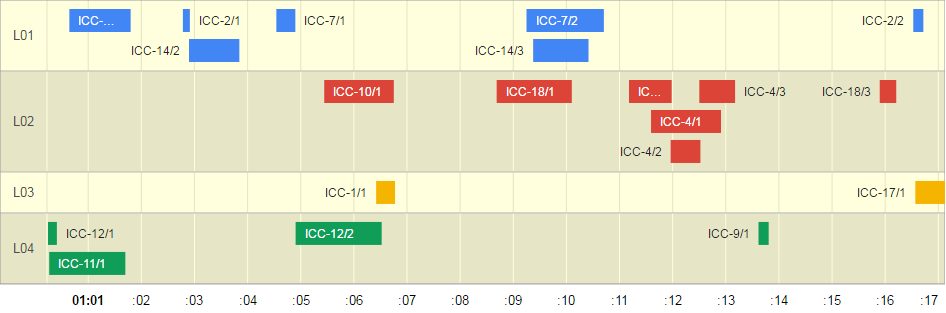
\includegraphics[width=0.75\textwidth]{figures/example-problem.png}
\caption{An example problem $P_1$}
\label{fig:example-problem-1}
\end{figure}


That problem instance $P$ directly defines also a schedule $\sigma_0$ based on the desired start times that is correct, if no devices in $D$ are incompatible, i.e. $I_0 = \emptyset$. 
This schedule however is not correct anymore, if we consider the incompatibility relation $I_1$ in which every device $L \in D$ is incompatible with itself. A correct schedule $\sigma_1$ for this incompatibility relation is shown in Figure~\ref{fig:example-solution-1}.

\begin{figure}[h]
  \centering
    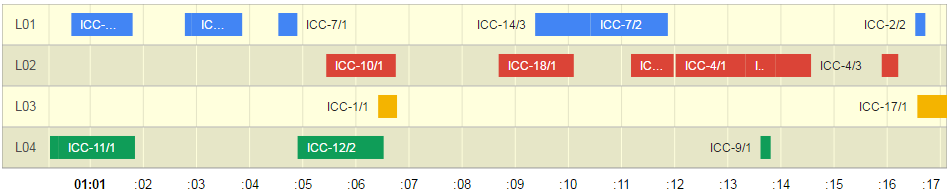
\includegraphics[width=0.75\textwidth]{figures/example-solution-self-incompatibility.png}
\caption{A correct schedule for the problem instance $P_1$ and incompatiblity relation $I_1$}
 \label{fig:example-solution-1}
\end{figure}


\paragraph{Example 2}
Fig.~\ref{fig:example-problem-2} is an example of a problem instance $P_2$ with four devices $D = \{L_1,L_2,L_3,L_4\}$, 20 output jobs and their desired start times.

\begin{figure}[!h]
  \centering
    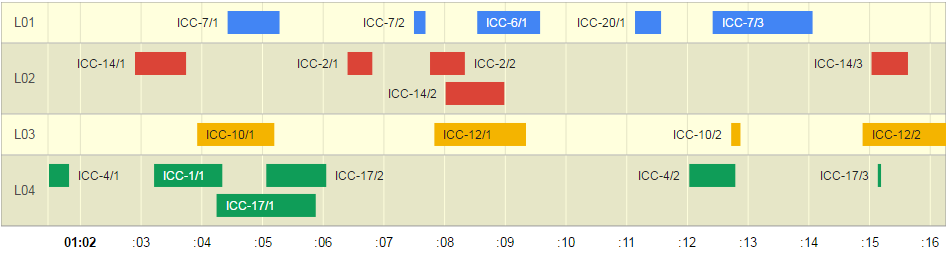
\includegraphics[width=0.75\textwidth]{figures/example-problem-2.png}
\caption{An example problem $P_2$}
\label{fig:example-problem-2}
\end{figure}

Consider the incompatiblity relation $I_2$ that defines that any two devices that are adjacent to each other in the scheduling table shown in Fig.~\ref{fig:example-problem-2} are incompatible with each other, e.g. $L_3$ is incompatible with all of $\{L_2,L_3,L_4\}$, but $L_1$ is not incompatible with $L_4$ for instance.   A correct schedule $\sigma_2$ for $P_2$ with incompatiblity relation $I_2$ is shown in Figure~\ref{fig:example-solution-2}.

\begin{figure}[h]
  \centering
    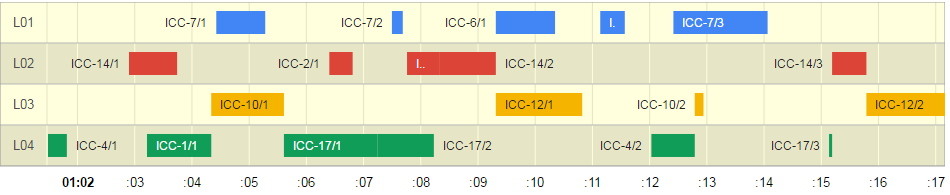
\includegraphics[width=0.75\textwidth]{figures/example-solution-adjacent-or-self-incompatibility.png}
\caption{A correct schedule for the problem instance $P_2$ and incompatiblity relation $I_2$}
\label{fig:example-solution-2}
\end{figure}



\paragraph{}
The respective decision problem to the optimization problem can be defined as follow: 

\begin{mydef}[{\sc output job Scheduling} Decision Problem]
\label{def:ic-scheduling-dp}
Given a finite  set ${C} = \{c_1, \ldots, c_n\}$ of output jobs, a finite set of  device names $D = \{d_1, \ldots, d_k\}$, total functions 
\begin{itemize}
\item[-]  ${start} : C \rightarrow \Nats_0$ for desired start times,
\item[-]   ${duration} : C \rightarrow \Nats_0$ for the expected output duration,  
\item[-]   ${device} : C \rightarrow D$ for the target output device
\end{itemize}
and an incompatibility relation $I \subseteq D \times D $, and a constant $q \in \Nats_0$, 
find a total function $\sigma: C \rightarrow \Nats_0$  called {\em schedule} that satisfies all of the following (correctness) constraints:
\begin{itemize}
\item[-]   ${start}(c) \leq \sigma(c)$ for all $c \in  C$, and
\item[-]  for all $c_1, c_2 \in C$ whenever $c_1 \not= c_2$ and $I({device}(c_1),{device}(c_2))$ then  $c_1$ and $c_2$ are non-overlapping in $\sigma$, i.e. $\sigma(c_1) + {duration}(c_1) \leq \sigma(c_2)$ or $\sigma(c_2) + {duration}(c_2) \leq \sigma(c_1)$
\end{itemize}
and the solution quality constraint:
\[{delay}(\sigma) = \sum_{c \in C} (\sigma(c) - {start}(c)) \leq q \]
ensuring that the total delay of output jobs in the schedule $\sigma$ in regards of the desired start times does not exceed the given bound $q$.

\end{mydef}

Note, that a correct schedule to the output job scheduling problem always exists: simply schedule all contexts one after the other (in some arbitrary order) such that at any point in time at most one output job is being active and all output jobs are being scheduled only after the desired start time. For later, we observe that the special case where all desired start times are $0$ and the expected output duration is $1$ any permutation of $C$ defines a correct schedule of length $n$ when scheduling the $i$-th element in the permuation at time $i$.

\section{Computational Complexity}
\label{sec:complexity}
In this section, we investigate the computational complexity of the output job scheduling problem (see Def.~\ref{def:ic-scheduling}). We will show that the optimization version of the problem is {\bf NP}-hard~\cite{GareyJohnson:CI:1979} by constructing a polynomial time reduction from {\sc Indendent Set} to {\sc output job Scheduling}. We also show that the decision problem is {\bf NP}-complete by a polynomial-time reduction of the optimization version of that problem.


\begin{mydef}[{\sc Independent Set}]
\label{def:independent-set}
Given a finite undirected graph $G = (V,E)$ and some integer $k \leq |V|$ determine if there is an {\em independent set} $S \subseteq V$  of size $|S| \geq k$, i.e. a set $S$ such that for all $v_1, v_2 \in V$ there is no edge in $E$ that connects $v_1$ and $v_2$.
\end{mydef}


%\begin{mydef}[{\sc Independent Set for Graphs without Loops}]
%\label{def:independent-set}
%Given a finite undirected graph $G = (V,E)$ without loops, i.e. there is no node $v \in V$ that is self-connected by some edge, and some integer $k \leq |V|$ determine if there is an {\em independent set} $S \subseteq V$  of size $|S| \geq k$, i.e. a set $S$ such that for all $v_1, v_2 \in V$ there is no edge in $E$ that connects $v_1$ and $v_2$.
%\end{mydef}

\begin{mylemma} \label{thm:independent-set-is-np-complete}
{\sc Independent Set} %and its restriction{\sc Independent Set for Graphs without Loops}  are 
is  {\bf NP}-complete. 
\end{mylemma}

\cite{GareyJohnson:CI:1979, 1994-papadimitriou} both give a proof of {\bf NP}-completeness of {\sc Independent Set}. The proof in \cite{1994-papadimitriou} constructs a polynomial-time reduction of {\sc 3-SAT} to {\sc Independent Set}. %which creates a loop-less undirected graph. Hence, {\sc Independent Set for Graphs without Loops} also is {\bf NP}-complete. 


\begin{mythm}
\label{thm:ic-scheduling-optimization-problem-is-NP-hard}
The {\sc output job Scheduling} optimization problem is {\bf NP}-hard.
\begin{proof}
We will proof the theorem by constructing a polynomial time reduction from {\sc Independent Set} to {\sc output job Scheduling}: 
Let $P = (G, k)$   be  instance of {\sc Independent Set} with a graph $G = (V,E)$ consisting of vertices $V$ and edges $E$. 

Based on $P$ we construct a corresponding instance $P^*$ of the optimization version of {\sc output job Scheduling} by setting 

\begin{itemize}
\item[-] the set of output jobs $C :=  V$ 
\item[-] the set of device names $D := V$
\item[-] the desired start times ${start}(c) := 0$ for all $c \in C$ ,
\item[-] the he expected output duration  ${duration}(c) := 1$ for all $c \in C$  
\item[-] the target output device ${device}(c) := c$ for all $c \in C$ 
\item[-] and the incompatibility relation $I := E$
\end{itemize}

%For some set $S$ and a function $f: S \rightarrow T$ we write $f(S)$ for the range of $f$ on $S$, i.e. $f(S) = \{ t \in T \,|\, f(s) \in s \in S\} \subseteq T$. 

\paragraph{}
The mapping from $P$ to $P^*$ takes linear time in the size of $P$. We now show that the mapping is also a reduction from {\sc Indendent Set} to {\sc output job Scheduling}, i.e.  it satisifes the following property  ($\ast$): 
\begin{center}
$P$ contains an indenpendent set $S$ of size at least $k$ if and only if an optimal solution $\sigma^*$ to $P^*$ schedules the output of at least $k$ output jobs in parallel. 
\end{center}

\paragraph{}
First, we proof the implication from right to left (,,if''):  Let  $\sigma^*$ be an optimal solution to $P^*$ that schedules the  output of at least $k$ output jobs in parallel, i.e. there exists some $t \in \{0, \ldots, |V-1| \}$ such that ${parallel}(\sigma^*, t) := \{  c \in C  \, |\,   {start}(c) = t  \ in\  \sigma^*\}$  has at  least size $k$. Since any two different elements in $c,c' \in {parallel}(\sigma^*, t)$  overlap with each other in  $\sigma^*$ and this schedule  is correct for $P^*$ it must hold that for any two different elements in $c,c' \in {parallel}(t)$ the respective devices ${device}(c) = c$ and   ${device}(c') = {c'}$ are not incompatible in $I$, hence $c$ and $c'$ are not connected in $E$. Therefore, ${parallel}(\sigma^*,t)$ is an independent set in $G$ of size at least $k$.

\paragraph{}
Next, we proof the implication from left to right (,,only if''):  Let $S$ be an independent set in $G$ with size at least $k$ and $\sigma^*$ be an optimal solution for $P^*$. 

We can observe the following: for {\em any optimal} solution $\sigma$ of $P^*$ it must hold that
\begin{enumerate}
\item All sets ${parallel}(\sigma, t)$ are independent sets in $G$ for $t \in \{0, \ldots, |V|-1\}$
\item All sets ${parallel}(\sigma, t)$ are either maximal independent sets in $G$ or for all $c \in C$ such that ${parallel}(\sigma, t) \subset {parallel}(\sigma, t) \cup \{c\}$ is an independent set  in $G$ there exists a $t' < t$ such that $c \in {parallel}(\sigma, t')$   (i.e. either they are maximal , or all possible output jobs that would cause an extension of the set to a maximum independent set in $G$ are already scheduled earlier in $\sigma$). 
\item The set ${parallel}(\sigma, 0)$ is a maximal independent set in $G$
\item For any $t,t' \in \{0, \ldots, |V| - 1\}$ such that $t \leq t'$:  ${parallel}(\sigma, t)$ contains at least as many elements as ${parallel}(\sigma, t')$.  Thus, the sequence of sizes of the output jobs scheduled at time $t=0,1,\ldots$ is monotonically decreasing.
\item The set ${parallel}(\sigma, 0)$ is a maximum independent set in $G$

%\item Any other optimal solution $\sigma'$ to $P^*$ will create the same sequence of parallelism, i.e. $ |{parallel}(\sigma, t)| = |{parallel}(\sigma', t)|$ for $t = 0,\ldots, |V|$ than $\sigma^*$ (in other words, the histogram of the output jobs being active at the same time is a unique fingerprint for all optimal solutions)
%\item For any  maximal independent set $M$ in $G$ there exists a ${parallel}(\sigma, t)$ such that $ |{parallel}(\sigma, t)| = |M|$
\end{enumerate}

\paragraph{}
The first item holds because $\sigma^*$ is a correct schedule wrt. the incompatiblity relation $I$ defined in $P^*$ (applying the same argument as above in the ,,if'' part of property ($\ast$)). 

To show the second item, we know because of the first item that all  ${parallel}(\sigma, t)$ are independent sets for all $t$. If ${parallel}(\sigma, t)$  is maximal, the statement holds. So lets consider the case that ${parallel}(\sigma, t)$ is not maximal in $G$. Then, there exists  $c \in C$ such that ${parallel}(\sigma, t) \subset {parallel}(\sigma, t) \cup \{c\}$ is an independent set in $G$. Consider any such $c \in C$. Since $c$  is scheduled in $\sigma$, $c$ has to be scheduled either before or after $t$. If it would be scheduled at time $t'$ later than $t$ in $\sigma$, then $\sigma$ would not be an optimal solution since we could strictly reduce the total delay by moving $c$ in $\sigma$ to start at time $t < t'$. Thefore, any such $c$ has to be scheduled strictly before $t$ in $\sigma$. Thus, the statement of the second item holds.

The third item follows immediately from the second item. 

The fourth item is also simple to show: assume that for some $t < t'$ we would have ${parallel}(\sigma, t)$ contains less elements than ${parallel}(\sigma, t')$. Then we could simply construct a schedule $\sigma'$ that switches the output jobs to be output at times $t$ and $t'$  and thus we would have a $\sigma'$ with ${parallel}(\sigma', t) = {parallel}(\sigma, t')$ and ${parallel}(\sigma', t) =  {parallel}(\sigma, t')$. Since then ${parallel}(\sigma', t)$ is smaller than ${parallel}(\sigma', t')$ and otherwise $\sigma$ and $\sigma'$ are the same, we constructed a schedule $\sigma'$ that has a smaller total delay ${delay}(\sigma') < {delay}(\sigma) $ than $\sigma$, which contradicts that $\sigma$ is an optimal solution (wrt. the total delay). Therefore, the assumption must be wrong and the statement of item four holds. 

It remains to show the last item:  
%We construct a ,,compact'' (thus low-cost) schedule $\sigma_{s}$ iteratively as follows:  We start with $i := 0$ and graph $G_i = G$.While $G_i$ contains an independent set , we pick a maximum independent set $M_i$ in $G$ and schedule it $\sigma_{s}$ at time $i$. Then, we construct $G_{i+1}$ from $G_i$ by removing from $G_i$ all vertices in $M_i$ and edges that start or end in $M_i$ and continue with $i := i+1$. The loop will terminate after finitely many steps (since in each step we remove at least one node from $G_i$), say when $i = j$.  Then, $G_j$ will be empty, since otherwise (by construction of our algorithm) $G_j = (V_j, E_j)$ will only contain self-loops, i.e. nodes $v$ such that there is an $E$-edge that connects $v$ with itself $v$ only. Those nodes and loops would also exist in the original input graph $G$ which contradicts that the graph dos not contain any vertices with self-loops.
%The resulting schedule $\sigma_{s}$ is a correct schedule for $P^*$ since in each step it schedules an independent set $M_i$ in $G$. 
%It also schedules at each step a maximal independent set in the graph $G_i$ which satisfies therefore also the second item above. In fact, it satisfies all other conditions and we should be able to show that it is in fact an optimal solution. If so, then the histogram of parallelism is unique to optimal solutions.
Assume that ${parallel}(\sigma, 0)$ is not a maximum independent set in $G$. Because of the third item above, we know that ${parallel}(\sigma, 0)$ is a maximal independent set. Hence, there exists a maximal independent set $M$ in $G$ that has more elements than ${parallel}(\sigma, 0)$.  So, in schedule $\sigma$ a smaller set than $M$ is scheduled at time $0$. and  $ |M| > |{parallel}(\sigma, 0)|$. With the fourth item above, we also have $|M| > |{parallel}(\sigma, t)|$ for all $t \in \{0, \ldots, |V| -1 \}$. Hence, the maximum indendent set $M$ cannot be scheduled in $\sigma$  as one set, but it is partitioned into parts $M_0,\ldots, M_{|V|-1}$ (some of which may be empty) such that $|M_t| < |{parallel}(\sigma, 0)|$ and $\cup_t M_t = M$ and $M_t \cap M_{t'} = \emptyset$ for all $t, t \in \{0, \ldots, |V| -1\}$ and $t \not= t'$ . 


We construct a schedule $\sigma'$ from $\sigma$ as follows: Select the smallest $j > 0$  such that $M_j$  is a non-empty partition of $M$.  Now, schedule all output jobs that are scheduled at time $0$ in $\sigma$ at time $j$ in $\sigma'$. Then,  schedule alle output jobs in $M$ at time $0$ in $\sigma'$. We schedule at time $t \geq 1, t \not= j$ in $\sigma'$ all output jobs that are scheduled at time $t$ in $\sigma$ and that are not also elements in $M_t$. 

The new schedule $\sigma'$  schedules all output jobs that have been scheduled by $\sigma$ and it is a correct schedule for $P^*$ too. Further, it has a smaller total delay than $\sigma$:  Since  $|M| > |{parallel}(\sigma, 0)|$ we schedule now strictly more output jobs at time $0$, i.e.  $|M| = |{parallel}(\sigma', 0)| > |{parallel}(\sigma, 0)|$. Compared to $\sigma$, we delayed $|{parallel}(\sigma, 0)|$ by $j$ time units, so we increase total delay in $\sigma'$ compared to $\sigma$  by  $j \cdot |{parallel}(\sigma, 0)|$.  At the same time, we decrease the total delay by $|M| \cdot j$ because (i) $\cup_j M_j = M$ , (ii) we schedule all elements of $M$ at time $0$, and (iii) all of these elements have been scheduled at time $t \geq j > 0$ in $\sigma$. The difference ${delay}(\sigma') - {delay}(\sigma) = j \cdot ( |{parallel}(\sigma, 0)|  -  |M| ) < 0$ is smaller than zero and therefore, $\sigma'$ has a smaller total delay than $\sigma$.  This contradicts that $\sigma$ is optimal. Hence, our assumption is wrong and ${parallel}(\sigma, 0)$ is  a maximum independent set in $G$.

\paragraph{}

Using these properties of optimal solutions, we can complete the proof of the implication by showing that in $\sigma^*$ there exists a ${parallel}(\sigma^*,t)$  such that $k \leq |S| \leq |{parallel}(\sigma^*,t)|$: we know that ${parallel}(\sigma^*,0)$ is a maximum independent set in $G$, hence it is at least as big as the independent set $S$ and therefore $k \leq |S| \leq |{parallel}(\sigma^*,t)|$ for $t = 0$.

\paragraph{}
Using property ($\ast$)  we can then construct an algorithm to reduce {\sc Independent Set} in polynomial time and correctly decide the original problem for all problem instances based on an optimal output job scheduling algorithm: Given $P$ we compute $P^*$ in polynomial time, then compute an optimal solution $\sigma^*$ to the corresponding information scheduling problem $P^*$. Then we give an answer to the original problem: we return "yes" for $P$ if and only if the computed optimal solution $\sigma^*$ for $P^*$ schedules the output of at least $k$ output jobs in parallel. The latter requires to compute ${parallel}(\sigma^*,0) = \{  c \in C\,  |\,  {start}(c) = 0 \ in\  \sigma\}$ and test if the set contains at least $k$ output jobs. This takes at most $O(n$) many additional steps. So overall, we have construct a polynomial time reduction that we aimed for. Because of Lemma~\ref{thm:independent-set-is-np-complete}, the optimal output job scheduling problem is therefore {\bf NP}-hard.
\end{proof}
\end{mythm}

\paragraph{Observations.} In fact, the proof shows that the optimization problem is already {\bf NP}-hard when we do not consider 
\begin{itemize}
\item[-]  individual release times for output jobs (i.e. all desired start times are the same, e.g. 0, hence no specific individual constraint to meet for the scheduler for each output job)
\item[-]  individual expected output durations for the output jobs (i.e. when we consider only output jobs with unit output length)
\end{itemize}

Further, the incompatibility constraints $I$ are a crucial source of complexity:  If we consider $I = \emptyset$, the problem becomes trivial and can be solved in linear time: simply output schedule $\sigma_0$ as defined by the individual desired output dates for output jobs, since this schedule  has ${delay}(\sigma_0)$ = 0 and thus clearly is an optimal solution.

\paragraph{}
Based on Theorem~\ref{thm:ic-scheduling-optimization-problem-is-NP-hard}, we can proof the {\bf NP}-hardness of the respective decision problem:

\begin{mylemma}
\label{thm:ic-scheduling-decision-problem-is-NP-hard}
The {\sc output job Scheduling} decision problem is {\bf NP}-hard
\begin{proof}
We construct a polynomial-time reduction of the {\sc output job Scheduling} optimization problem to the {\sc output job Scheduling} decision problem: 

We can always construct a correct and complete schedule for a problem instance $P$ of the {\sc output job Scheduling} problem by scheduling output jobs sequentially, i.e. one after another such that no two output jobs overlap in time and  between any two output jobs that have been scheduled, there is not gap between them. Thus, the maximal possible total delay for any correct schedule is at most
\[ D =n ({max}_{c \in C}{start}(c)  + (n-1) {max}_{c \in C}{duration}(c)) \]
since for each of the $n$ output jobs that are scheduled, there are at most $n-1$ output jobs scheduled before,  each can cause at most a delay of ${max}_{c \in C}{duration}(c)$ and we safely begin to schedule all output jobs after the latest desired start time to satisfy all start time constraints in $P$. 

Thus, there are only finitely many possible upper bounds $q$ on the quality of correct schedule $\sigma$  to consider, i.e. $q \in \{0,\ldots, D\}$. We can perform binary search on  $q \in \{0,\ldots, D\}$ using the algorithm to solve the {\sc output job Scheduling} decision problem for the given problem instance $P$ with quality bound $q$ in order to find the smallest value $q^*$ such that there exists a correct schedule $\sigma^*$ for $P$ that satsfies the quality bound $q^*$  in $O(log(D))$ search steps. This is possible because of the monotonicity of the decision problem: if there is a correct schedule $\sigma$  with a total delay ${delay}(\sigma) \leq q$, then we can infer that the same holds for all $q' \geq q$; on the other hand, if there is no correct schedule $\sigma$  with a total delay ${delay}(\sigma) \leq q$, then we can infer that the same holds for all $q' \leq q$ too.

 This allows us to compute an optimal schedule $\sigma^*$ in at most polynomialy many calls (in regards of the size of the input problem $P$) to the decision procedue for the {\sc output job Scheduling} decision problem. Therefore, we have a polynomial time reduction of the optimization problem to the decision problem. Since, the optimization problem is {\bf  NP}-hard, the decision problem is {\bf NP}-hard too.
\end{proof}
%\begin{proof}
%Given a  problem instances $P$ of the {\sc output job Scheduling} decision problem with quality bound $q$, we reduce it %to solving  the optimization problem as follows: 

%Consider $P$ without the quality bound $q$ and solve the optimization problem for this instance. Given the optimal schedule $\sigma^*$ computed by an algorithm $A$ to solve the optmization problem, we can simply compute the solution quality $q^*$ of the optimal schedule $\sigma^*$ in linear time and solve the decision problem by returning "yes" if and only if  $q^* \leq q$.

%This clearly is a polynomial time reduction from the decision problem to the optimization problem. Because of Lemma~\ref{thm:ic-scheduling-optimization-problem-is-NP-hard}, the decision problem of {\sc output job Scheduling} is then also {\bf NP}-hard.
%\end{proof}
\end{mylemma}


\begin{mylemma}\label{thm:ic-scheduling-decision-in-NP} 
{\sc Output Job Scheduling} decision problem is in {\bf NP}.
\begin{proof}
Given an instance $P$ of the {\sc output job Scheduling} decision problem with a quality bound $q$, we can observe:

For all $c\in C$ the candidate sets for $\sigma(c)$ are subsets of $\{ 0, \ldots, D\}$ for the value $D$ defined in the proof of Lemma ~\ref{thm:ic-scheduling-decision-problem-is-NP-hard} above and therefore finite. Hence there are only finitely many candidate schedules $\sigma$ to consider. Given a candidate schedule $\sigma$, we can verify the conditions for correctness of the schedule from Def.~\ref{def:ic-scheduling} in polynomial time with respect the problem instance size (assuming unary coding of numbers). Therefore, we can define a non-deterministic Turing machine that first guesses non-deterministically a candidate schedule $\sigma$ and then checks in polynomial time for correctness of the schedule and if the upper bound on the solution quality $q$ is met by the schedule. If that is the case, the machine stops and accepts the input $P$. Otherwise, the machine does not accept the input.
\end{proof}
\end{mylemma}


Given Lemma~\ref{thm:ic-scheduling-decision-problem-is-NP-hard} and Lemma~\ref{thm:ic-scheduling-decision-in-NP} , we have shown 


\begin{mythm}
The {\sc Output Job Scheduling} decision problem is {\bf NP}-complete.
\end{mythm}

\begin{mycor}
Any restricted class $\mathcal{G}$ of graphs for which {\sc Independet Set} is {\bf NP}-hard,  the {\sc output job Scheduling}  is  also {\bf NP}-hard when restricting the device incompatibility relation to graphs in $\mathcal{G}$. 
\begin{proof}
Our proof of Theorem~\ref{thm:ic-scheduling-optimization-problem-is-NP-hard} and Lemma~\ref{thm:ic-scheduling-decision-problem-is-NP-hard} constructs a reduction that does not change the input graph of the {\sc Independent Set} instance considered. Hence, it applies in the same way for any restricted class of graphs for which {\sc Independent Set} is {\bf NP}-hard.
\end{proof}
\end{mycor}

This allows us to directly identify many more restricted cases, where the output job scheduling problem already is {\bf NP}-hard~\cite{GareyJohnson:CI:1979}, for instance cubic planar graphs, total graphs of bipartite graphs, and graphs containg no triangles.

%\section{Approximating Optimal Solutions}
%\label{approximation}

%\section{Conclusions}
%\label{conclusions}

\bibliography{scheduling}
\bibliographystyle{plain}


\end{document}
